\section{Design}
\subsection{Overview}
We design a framework named \sysname which integrates in-network computation with the DML framework. A \sysname application job trains a model with several workers and one PS. After training one batch of data points,  each worker generates a local gradient, and all workers and the PS has two phases to update parameters. In the first phase, each gradient traverse a path to the PS, and all paths form a tree structure in the network topology; in the second phase, the PS accumulates all gradients to the parameters locally at the PS (with a learning rate), and broadcasts the updated parameters to each worker.

\sysname deploys an aggregation service on the programmable network switches (undertaken by a few strcuctures named aggregators). In phase 1, whenever the two or more bytestreams of the gradients from the same ML application instance meet in the switch, they are aggregated; in this way, network traffic volumes is reduced and PS aggregation computation is offloaded, and the ML application get performance gain (\textbf{R2}). The aggregation service on each switch has a maximum fan-in degree (many-to-one), but all involved switches on the aggregation tree are organized in a hierarchical structure, supporting the system to scale up (\textbf{R3}). To simplify the switch configure (\textbf{R4}), the aggregation service is isolated from other configurations (routing, firewall, etc.) on the switch, once \sysname traffic is recognized by a classifier, they would traverse the aggregation service. And the aggregation service is \emph{best-effort} --- if an aggregator cannot get complete aggregation result due to some worker's failure (e.g., packet loss, machine failure), it would send partial results. In phase 2, the switch employs a broadcast mechanism to duplicate one copy of updated parameters to many workers.

On the workers, \sysname reconstructs the network stack for the in-network service. \sysname wraps up the same tensor sending/receiving interfaces as existing frameworks (e.g., BytePS, PyTorch) so that it is compatible with existing frameworks (\textbf{R5}). As the swtiches only provide a best-effort service, the workers and the PS (\sysname network stack) coordinate to guarantee the logical correctness (\textbf{R1}). In Phase 1, when a worker sends a packet stream of its gradient, each packet also encodes the aggregation information; the switches does not guarantee a complete aggregation result: if packets are not lost but not aggregated, the PS would continue the aggregation (based on the aggregation information in packets) and compute the complete result, if packets are lost, the PS would send acknowledged parameter packets to trigger retransmission on the workers. In the design and implementation, we overcome the following to challenges.

\textbf{(C1) Supporting flexible aggregation structure.} In a multi-tenancy network, we assume the applications can be deployed flexibly in the network, thus the gradient aggregation tree can be of arbitrary structure from multiple workers to one PS. While the network topology is fixed, in different trees, one specific program switch may be at different positions and hierarchies, and in charge of aggregating gradients from different potions of workers. It is challenging to make an application-agnositic switch work correctly for all possible application deployments.

\textbf{Solution:} \sysname uses the deployment plan (i.e., worker and PS location) and the network topolgoy (including programmable switches) to pre-compute the aggregation tree, and then it pre-computes the aggregation services for each worker's gradient and encodes this information (aggregation hierarchy) into the gradient packet header. Each on-path programmable switch would behave according to its own aggregation hierarchy: dropping duplicated packets, sending completely aggregated result, and handling retransmitted packets.




\wenfei{write until here}

\textbf{(C2) Enforcing efficient switch resource sharing.} In existing networked applications, when different instances compete for network bandwidth, congestion control is usually used to let each part backoff and converge to a global stable state, where network bandwidth is efficiently utilized with high saturation. In \sysname, there is one more kind of resource for \sysname instances to compete for --- the aggregators on programmable switches. 



In a multi-tenancy network, several ML applications and non-ML applications coexist, all application instances may contend for various network resources --- the instances of both ML and non-ML applications may contend for network bandwidth, ML application instances may contend for aggregator on switches. A machanism is needed to avoid network resources is efficiently used (i.e., not wasted and not abused). It is challenging to design one uniform mechanism solve various possible contentions.

\textbf{Solution:} We analyze three possible reasons of contention --- link bandwidth, switch aggregators, and receiver 





\textbf{(R7) Efficient Resource Sharing.} Network resources such as bandwidth and switch memory (for in-network computation) are shared among multiple ML and non-ML applications. Once contention happens, all contending applications should coverge to a stable state where network resources are efficiently used without being abused or wasted.


\textbf{(R5) topology freedom.} Similarly, a network topology could vary from network to network. An in-network computation solution should be deployed and work without assuming the network topology.


Recent success of the in-network computation has attracted more 
applications to be arised.  
\TODO{talk about the machine learning system.}
\TODO{Talk about traffic pattern: multiple workers and one parameter server.}

\switchml introduces in-network aggregation for machine learning systems
to speed up the training. The benefits from in-network computation 
come from two sides: (1) reduce network traffic; (2) reduce the computation
at the parameter servers. 
It employs a programmable switch as the parameter server instead of a host. 
\switchml targets on the rack scale. We also argue that using programmable switch
as the parameter server limits \switchml to be scaled up to 
thousands of nodes. A system which can be deployed to thousands of nodes requires:


(1) a congestion control protocol that can support the system to
co-locate with other applications, which does not use the in-network computation feature;
Isolating their traffic to the normal traffic is the state-of-the-art methodology to 
address this issue in the recent proposed in-network computaiton system~\cite{netcache, netchain, harmonia, switchml}, which wastes the network resources. 
A distributed system running in a large cluster requires the underlying networking stack equipped with 
congestion control mechanism such that they can share the network
bandwidth fairly or according to pre-configured policy.
In addition, it also requires the packet loss recovery mechanism to ensure 
reliability. Congestion collapse can happen due to the lack of congestion control, 
which finally result in low network goodput, i.e., the longer job completion time. 
The broken of the end-to-end semantics impends the congestion control mechanism to implement
in this kind of the in-network computation systems. 


(2) a resource sharing scheme that different machine learning systems/jobs
are able to share and maximally utilize the network resources, i.e., in-network computation;
To share the switch computation resources, i.e., the memory, we can pre-allocate 
the resources before a job starts, i.e., 
the memory location in switch that each packet should access, and the
size of the memory that one job can be used are fixed during the running time.
However, the machine learning jobs are running in thousands of iterations, 
the network communication
follows the classic on-off traffic pattern. The resources pre-allocated to 
a job is wasted when the job is in an communication off mode.
To maximally utilize the switch computation resources, 
the system is able to dynamically adjust resource utilization in
the dataplane when another new in-network application enters into the network.
The difficulty to achieve this goal lies on that the switch program can not dynamically 
allocate the memory in the data plane after the program starts.

(3) the system is able to be deployed to the whole data centers as
the training job size grows;
\TODO{say something that the model size grows and model becomes more sophisticated
and why do we need to support scalibility.}
We can view can reduction path from all the workers to the parameter servers as a tree structure.
The workers are the leaves, the parameter server is the root and the switches along the path 
is the node in the tree structure.
To deploy such in-network systems to the switch, it requires each hop of the switch 
to be carefully configured.
It adds the management complexity while the switch 
in the network also serves as packet switching for normal traffic.


\switchml can not achieve the above mentioned features as the programmable
switches has limited computation and memory resources.
\if 0
The state-of-the-art in-network applications use timeout to detect packet loss for the implementation ease. Packets loss recovery is a core component in
traditional TCP networking stack.
In TCP, each packet is marked by a monotonically increasing sequence number. 
If the receiver receives out-of-order packets, it sends an ACK packet with the lowest 
expected packet sequence number to the sender. 
When the sender receives three duplicated ACKs, it assumes a packet loss happens.
While a packet may be consumed at switch, it can cause the confusion at the receiver
that a packet loss happened. It is challenging to design loss recovery due to that the end-to-end semantics are broken 
for these new applications.
 
Finally, these in-network applications assume that the switch always has the resources to do the aggregation,
which is not true as more in-network applications enters into the network. Thus, it requires the applications or
the underlying protocol to be able to handle the best efforts case, where the network may or may not do the 
aggregation for the application. This relaxed the restriction that the in-network applications has to be deployed 
in a programmable switch or a switch has the in-network aggregation program loaded.   
\fi 
This motivates us to design a new architecture, called \system, to meet the following requirements such that it can (1) be capable with normal applications; (2) support dynamic resource sharing with in-network applications in the data plane;
(3) support large scale deployment; (4) be easily extended to a general framework that can used in other applications~\TODO{need more thinking.}. 

\system obeys the end-to-end principle and uses the end hosts as workers and parameter servers. 
The end-to-end principle enables us to implement the congestion control and packet loss recovery 
naturally at the end host. A straightforward approach could totally employ 
the congestion control and packet loss recovery from traditional TCP stack.
In TCP, each packet is marked by a monotonically increasing sequence number. 
If the receiver receives out-of-order packets, it sends an ACK packet with the lowest 
expected packet sequence number to the sender. 
When the sender receives three duplicated ACKs, it assumes a packet loss happens.
While a packet may be consumed at switch, it can cause the confusion at the receiver
that a packet loss happened. It is challenging to design loss recovery due to that the end-to-end semantics are broken even we still use the hosts as the end points as the traditional machine learning systems. 
 
Secondly, as the in-network aggregation requires maintaining the state in the switch, 
we need \TODO{need to be specific.}

Thirdly, the management complexity on the switch to deploy 
the in-network aggregation system on the whole data centers 
are still requires to be addressed.
\TODO{need more specific.}      



By resolving the above challenges, \system achieves the same performance benefit 
as \switchml in the rack scale. 
It is also able to be deployed in the large scale while improve the significant 
performance in the data center scale compared with traditional machine learning systems. 
Finally, it can be deployed both in the cluster with and without 
programmable switches and is capable to run with other \system traffic and normal traffic. 
\TODO{some experiments results.}

% overview and challenge
\begin{figure}[htb]
    \centering
    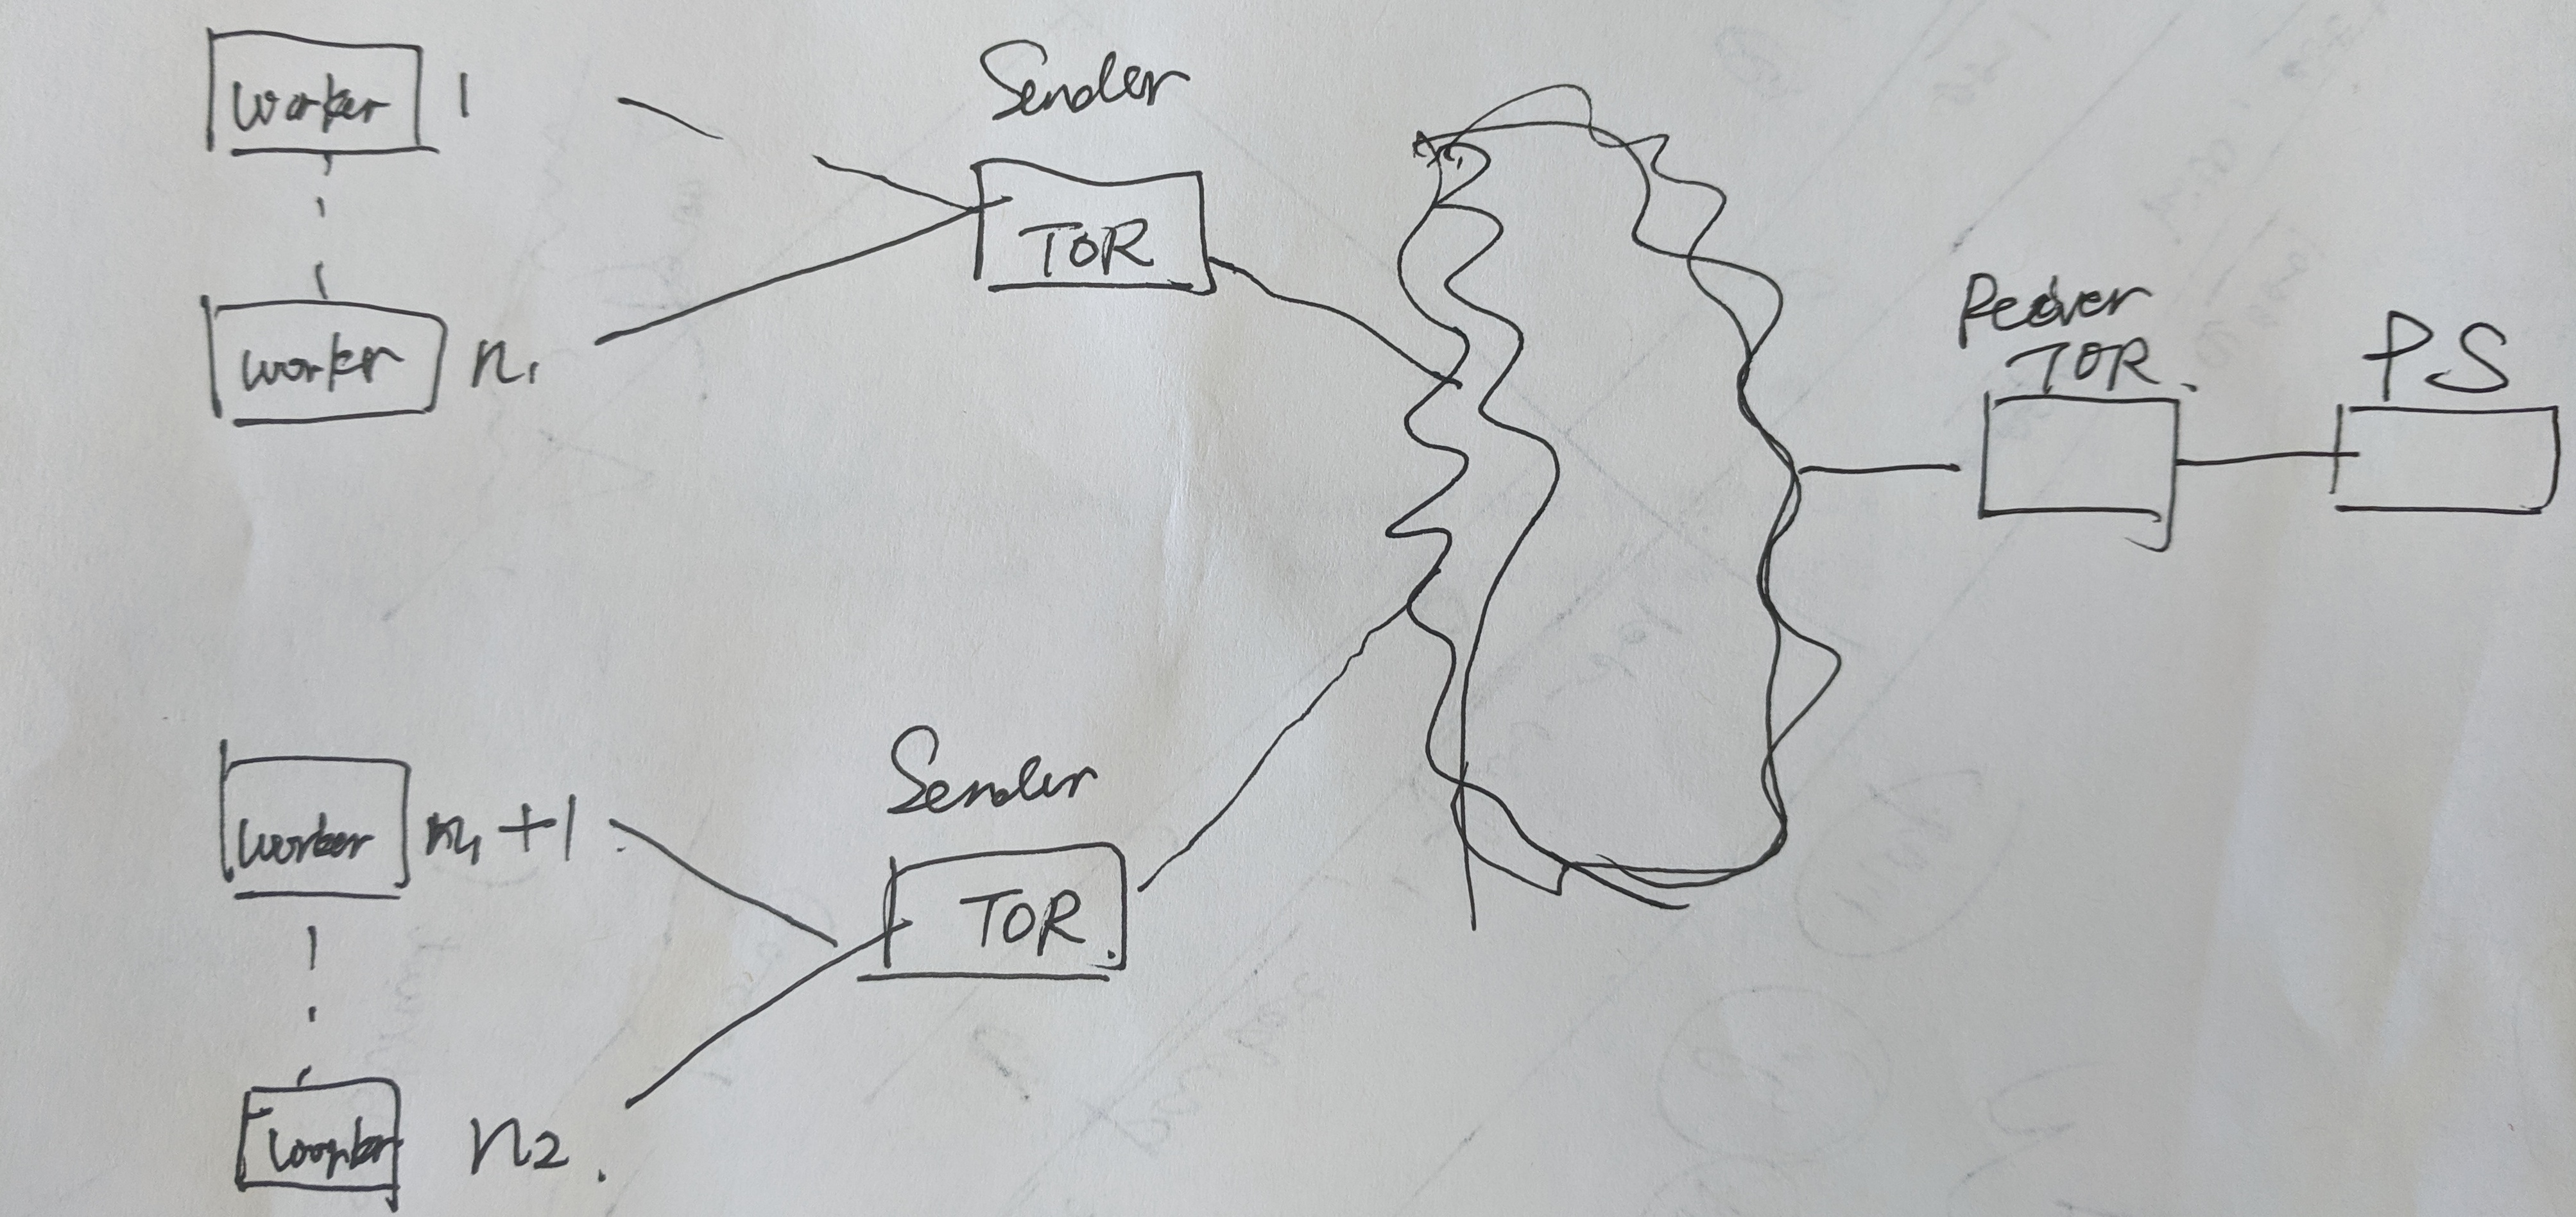
\includegraphics[width=1.0\linewidth]{figures/p4ml-arch.jpg}
    \caption{\system Architecture}
    \label{fig:p4ml-arch}
\end{figure}
\begin{figure}
    \centering
    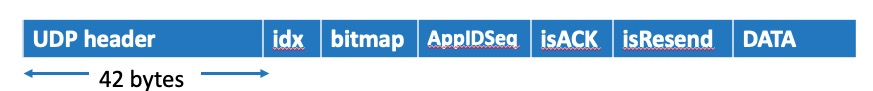
\includegraphics[width=1.0\linewidth]{figures/pktformat.jpeg}
    \caption{\system Packet Format}
    \label{fig:packet-format}
\end{figure}
\begin{table}[h!]
  \begin{center}
    \caption{Packet Fields.}
    \label{tab:packet-field}
    \begin{tabular}{|l|c|} 
	\hline
		\textbf{Field} & \textbf{Description} \\
      \hline
      idx & the aggregator position in switch.\\
      \hline
		bitmap & worker position within ToR switch. \\
      \hline
		AppIdSeq & Application ID and sequence number of a packet.\\
	  \hline
		isACK & 1, if it is the aggregation result packet, otherwise, 0. \\
		\hline
		isResend & 1, if it is a retransmitted packet, otherwise, 0. \\
		\hline 
		DATA &  128 bytes gradients value. \\
		\hline 
    \end{tabular}
  \end{center}
\end{table}
We propose \system, a in-network aggregation framework for machine learning systems.
Figure~\ref{fig:p4ml-arch} shows the architecture of \system. 
\system keeps the same architecture, workers and parameter server, as general machine learning systems
while has the aggregation functionality deployed in the ToR switches of the workers and parameter server.

In this architecture, workers do the computation, and transfer the gradients to parameter server.
via \system networking stack. The networking stack of \system packs the data into \system 
packet format, guarantees the reliability of packet delivery, and provides the congestion control
to achieve the high utilization of the link.
In addition for providing the basic switching to the traffic going through the switch, 
the switch also offers the aggregation between multiple packets and forwards the aggregation results
to the parameter server.
Finally, the parameter server receives the aggregation result, restores the aggregation results for persistency, 
and send the aggregation results after putting an ACK flag into the packet header.

The packet format is crucial for the communication between the switches and end hosts. 
We present \system packet format in Figure~\ref{fig:packet-format}, where the \system
control information is above the UDP header. The description of the fields is shown in
Table~\ref{tab:packet-field} and we will discuss how these fields are used 
to guarantee the correctness of the computation in the dataplane later in this section 
As aggregation operations are stateful operations, thus, we
need use register in the switch. The tofino switch has maximum of $12$ stages and each stages
can only process up to $4$ registers. As the control information presented in 
Table~\ref{tab:packet-field}, we finally take $8$ stages with each stage processing $4$ $32$-$bit$
integers, which results in total of $128$ bytes gradients value per packets.

\begin{algorithm}[ht!]
	\caption{\textbf{Function CleanSTATE($pkt$)}}
    \begin{algorithmic}[1]
			\IF {pkt.AppIdSeqnum == AppIdSeqnum[pkt.idx] }
			\STATE agg[pkt.idx] = 0
			\STATE bitmap[pkt.idx] = 0
			\STATE AppIdSeqnum[pkt.idx] = 0
			\STATE counter[pkt.idx] = 0
			\ENDIF
	\end{algorithmic}
    \label{func:stateclean}
    \end{algorithm}
\subsection{Basic Idea}~\label{basic-idea}
We begin by describing a basic idea, which only consider the aggregation in
switch within a rack~\footnote{Note that the design of basic idea is easy to extend to the full version of \system.}.
It assumes that (1) no packet loss; (2) the aggregator in switch is always available
whenever a packet from worker is sent to the switch;
(3) \system is the only traffic in the switch;
(4) the network is rack-scale.
We will show how the complete design of \system removes these assumptions in section~\ref{}-~\ref{}.

\subsubsection{Switch Logic}
\begin{algorithm}[ht!]
    \caption{ Switch Logic of Strawman solution}
    \begin{algorithmic}[1]
        \STATE \textbf{Initialization:}
		\STATE AppIdSeqnum[s]:={0}
		\STATE bitmap[s]:={0}
		\STATE agg[s]:= {0} 
        \vspace{4mm}
		\STATE {Extract packet fields pkt(idx, bitmap, forwarding, AppIdSeqnum, isACK, vector) }
		\IF {pkt.ACK == 0}
		\IF {AppIdSeqnum[pkt.idx] == 0}
		\STATE AppIdSeqnum[pkt.idx] = pkt.AppIdSeqnum
		\ENDIF
		\IF {pkt.AppIdSeqnum == AppIdSeqnum[pkt.idx] }
		\STATE bitmap[pkt.idx] = bitmap[pkt.idx] | pkt.bitmap
		\IF {(pkt.bitmap \textbf{\&} \textbf{NOT} bitmap[pkt.idx]) != 0}
		\STATE	agg[pkt.idx] = agg[pkt.idx] + pkt.vector
		\ELSE
		\STATE drop pkt
		\ENDIF
		\IF {bitmap[pkt.idx] == pkt.forwarding}
		\STATE  pkt.vector = agg[pkt.idx]
		\STATE  forward pkt to parameter server
		\ELSE
		\STATE drop pkt
        \ENDIF
		\ENDIF
		\ELSE
		\STATE CleanSTATE(pkt)
		\STATE multicast pkt
		\ENDIF
	%%	\ENDFUNCTION
	\end{algorithmic}
    \label{algo:strawman-scheduler-switch}
    \end{algorithm}
Switch has the core logic (shown in Algorithm~\ref{algo:strawman-scheduler-switch}) to provide the in-network computation.
The switch first allocates a big pool of memory when it starts and initialize 
the value as $0$ (line $4$ in Algo~\ref{algo:strawman-scheduler-switch}). This is because the switch dataplane can not 
allocate memory for the aggregation during run-time.

When a packet arrives to the switch, the 'idx' field in the packet header indicates the aggregator index at the switch.
The switch maintains a AppIdSeqnum for each packet to verify whether it is the right memory location to do the aggregation. 
Upon receiving a \system packet, the switch first check if the targeting aggregator is occupied. 
If not, it claims the usage of this aggregator (line 7-9 in Algo~\ref{algo:strawman-scheduler-switch}).
After validating that it is the right memory location to do the aggregation and check that the same packet has not been aggregated,
the switch updates the bitmap value to indicates the expected packets from this worker is done with the aggregation to guarantee
that the aggregation on the same packet happens exactly once (line 12-14 in Algo~\ref{algo:strawman-scheduler-switch}).
Finally, if the expected same sequence packets from all the workers are received, the switch writes the aggregation
results to the packet, and forward the packet to the parameter server; otherwise, it drops the packet (line 17-22 in Algo~\ref{algo:strawman-scheduler-switch}).

We use 'isACK' to indicates that this is a packet which contains the aggregation results.
The switch seeing the packet with 'isACK' set does not do aggregation, and instead 
clean all states for this packet, multicasts
this packet to all the workers (line 24-27 in Algo~\ref{algo:strawman-scheduler-switch}). 
The ideal moment to clean the state should happen when the aggregation is done. However, due to 
the limitation that the same memory region can not be visited twice in Tofino switch, we push 
this action when the parameter sent the aggregation results back to the worker.

\subsubsection{Packet I/O Efficiency}
The main challenge raised at the host side is the performance issue on small packets in the network is whether 
such in-network aggregation system can keep up with the line rate (i.e., 100Gbps) as CPU 
is the bottleneck for sending and receiving packets.
The state-of-the-art userspace networking programming models, e.g., RDMA, DPDK, Raw Ethernet
requires the CPUs of sender and receiver post packet descriptors to the NIC such
that NIC can do DMA read or write.

We pick the RAW Ethernet as userspace programming library. As you can see in Figure~\ref{fig:io-optimization},
without any hardware acceleration, we can only get the maximum throughput of 10Gbps in our packet IO
benchmarking with \system packet size. 
\yanfang{need a figure with 3 bars. sending/receiving packets in cpu: 10Gbps, with TSO at sender/receive in cpu: 34Gbps; with TSO at sender/mp-qp in receiver: 50Gbps.}


We find that commodity NICs, e.g., Mellanox RNICs, supports TCP Segmentation Offload~\footnote{Note it supports any packet format though the name refers to TCP packets.}, called TSO~\cite{}. TSO enables the NIC to accept 
large chunk of data with the size greater than MTU. The 
TSO engine at NIC splits the data into multiple packets with the 
user-specified packet size and inserts the user-specified headers per packet in NIC.
With TSO, CPU is released while the sending rate is increased due to this hardware offloading. 
As we can see the Figure~\ref{}, the throughput jumps to 35Gbps with TSO.

We found another advanced feature supported by the commodity NICs for the receiver side acceleration, 
called {\it multi-packet} RQ. MP-RQ can specific multiple contiguous packet buffers
using base address, buffer size, and number of buffers, which indicates the CPU can only post one packet descriptor while receiving multiple packets. With the default configuration of the $512$ packets per receive descriptor, 
\system is able to get around 50Gbps echo throughput with support of TSO and MP-RQ. 
We argue that this is the upper bound throughput per worker in a 100Gbps network in the distributed machine learning systems
as the link to the parameter servers is the bottleneck and shared by at least $2$ workers.



\subsubsection{Worker Logic and Parameter Server Logic}
The switch logic does not have knowledge for a packet to use which switch aggregator and how many aggregators to use.
The worker has to carefully set the aggregator position for each packet, such that
the expected packets go to the same aggregator to do the aggregation. 
In our setting, each aggregator can deal with 32 4-bytes integer. 
The total bytes that can be aggregated in the switch is (aggregator number * $128$ bytes).
In addition, the model size is large than the above limitation. 
We have to carefully split the model into small batches such that
the packet going through the switch has a chance to be aggregated. 
We set our default aggregator number as $100$ because this is the minimum switch
memory utilization but able to get the best performance on network I/O.
\yanfang{need mention streaming protocol.}
At worker side, we also start multiple threads to achieve high packet I/O rate.
When the \system library receives a model to transfer, it assigns to a thread to send.
Multiple threads can speed up the performance, however, it can cause the 
that the same model being assigned into different threads, which leads 
the packets to be aggregated from different workers can not meet in the same switch aggregator. 
In addition, it can also cause the unbalanced load between different threads, which degrades
the performance as the overall training performance relies on the slowest worker. 

\system has a centralized scheduler to receive the models from application layer 
and maintains the total load for each thread at each worker. 
Whenever the centralized scheduler receives a model to be transferred, it extract the size and 
assigns it to the least loaded thread. With this strategy, \system balanced the load
between threads while ensures that the same model from different workers is assigned to the same thread.


As \system is targeting on the lossy setting and multi-tenancy environment, 
\system use bitmaps to indicate the id of a worker in the job 
and identify whether the packet from the worker has been aggregated. 
This prevents a same model updates applied twice to the aggregator.
\system also uses the application id and the sequence number (i.e., `AppIdSeq` field) 
to claim the occupancy of a model update, which prevents the unexpected packets, 
e.g., the same sequence packet from different application, 
or the different sequence packet from the same application, are applied 
to the aggregator. 

Whenever the parameter server receives a packet, it sets the `isACK` bit and sends back to the switch.
%%\begin{algorithm}[ht!]
%%    \caption{\system Switch logic handling packet loss and resource sharing }
%%    \begin{algorithmic}[1]
%%        \STATE \textbf{Initialization:}
%%		\STATE AppIdSeqnum[s]:={0}
%%		\STATE bitmap[s]:={0}
%%		\STATE agg[s]:= {0}
%%        \vspace{4mm}
%%		\STATE {Extract packet fields pkt(idx, bitmap, forwarding, AppIdSeqnum, isACK, isResend, vector) }
%%		\IF {pkt.isResend == 1}
%%		\STATE CleanSTATE(pkt)\COMMENT{handle packet loss}
%%		\STATE forward pkt to parameter server
%%		\ELSE
%%		\IF {pkt.ACK == 0}
%%		\IF {AppIdSeqnum[pkt.idx] == 0}
%%		\STATE AppIdSeqnum[pkt.idx] = pkt.AppIdSeqnum
%%		\ENDIF
%%		\IF {pkt.AppIdSeqnum == AppIdSeqnum[pkt.idx]}
%%		\STATE bitmap[pkt.idx] = bitmap[pkt.idx] | pkt.bitmap
%%		\IF {(pkt.bitmap \textbf{\&} \textbf{NOT} bitmap[pkt.idx]) != 0}
%%		\STATE	agg[pkt.idx] = agg[pkt.idx] + pkt.vector
%%		\ELSE
%%		\STATE drop pkt
%%		\ENDIF
%%		\IF {bitmap[pkt.idx] == pkt.forwarding}
%%		\STATE  pkt.vector = agg[pkt.idx]
%%		\STATE  forward pkt to parameter server
%%		\ELSE
%%		\STATE drop pkt
%%        \ENDIF
%%        \ELSE
%%		\STATE forward pkt to parameter server \COMMENT{best effort, let PS handle}
%%		\ENDIF
%%		\ELSE
%%		\STATE CleanSTATE(pkt)
%%		\STATE multicast pkt
%%		\ENDIF
%%		\ENDIF
%%	%%	\ENDFUNCTION
%%	\end{algorithmic}
%%    \label{algo:scheduler-switch}
%%    \end{algorithm}


\subsection{CC and packet loss}
To share the network with the normal TCP/UDP traffic in the network,
congestion control is required to avoid packet loss and packet loss 
recovery is required to guarantee the reliability from networking stack.
Congestion control essentially has two goals: efficiency and fairness.
As \system merges multiple flows into one flow, it's hard to define whether 
the fairness should among the flows from workers or among the flow to the server.
We leave this debate to the audience.
Thus, the congestion control of \system aims to avoid packet loss such that 
the aggregate goodput can achieve the line rate for each link.

\system picks the ECN mark as the congestion control signal. 
The other well-known congestion control 
signal RTT,  measured from when a worker sends a model update packet until it gets the aggregation result packet.
We noticed that RTT is not right choice in this case due to the two main reasons:
(1) RTT can not reflect the network congestion, this is because per packet RTT
also includes the synchronization delay between workers.
(2) In addition, different workers get the different RTT measurement value.
A worker who sends the first packet of the aggregation gets higher RTT delay than a worker sends the last packet. This can cause the different sending rate from different workers. 
This can cause stragglers in the SGD computation and slow down the training speed.
Because ECN mark reflects the switch queuing size and all the workers receives the same aggregation packet, using ECN as the congestion signal can avoid the above problem.
After carefully choosing ECN as the congestion control signal,
\system uses window based scheme as \system's maximum window size
is only $25$KB per flow and wants to occupy the switch resources
at the same time.\yanfang{need more thinking about the above statement.}
\system adopts the classical AIMD as the congestion response and implements 
the congestion control as a totally end-to-end approach.

\yanfang{need more writing about the challenge.}
Recovery from packet loss requires the end host for retransmission.
\system uses the out-of-order packet sequence to detect a packet loss at the worker.
The worker marks the packet as the retransmitted packet. 
To reduce the complexity of the switch logic and pushing the complexity to the end host,
whenever the switch receives a packet with `isResnd` mark except the first resend packet, it cleans
out all the state maintained for the occupied switch aggregator (line 6-8 in Algorithm~\ref{algo:scheduler-switch}).

As a small optimization, when the switch receives the first resend packet, 
it first does the aggregation if it is not seen by the aggregator before, then, write the 
current partial aggregation result to that packet to reduce the computation at the parameter server.
Finally, it is forwarded to the parameter server.


\subsection{Full utilization of switch resources}
To support multi-tenancy scenario, i.e., concurrent \system jobs running at the switch, 
a straightforward solution would assign a separate memory pool of the switch before a job starts~\cite{switchml}.
This approach could not scale as the memory size is limited. For example, \switchml 
uses the $10$\% of the switch memory for a job, which limits at most $10$ jobs can get run concurrently to get 
the benefit of in-network aggregation. In addition, we noticed that the machine learning systems
follows the on-off traffic pattern in each iteration. 
\yanfang{need a figure to show this on-ff traffic pattern.}
That said the machine learning 
systems spend a period of time on computation, then, a period of time on communication
and loop this pattern until some metrics converge or the user decides to stop. 
This traffic pattern offers other jobs an opportunity to utilize the memory pool 
when a job is busy for the computation.

To get full utilization of the memory in the switch during the running time, 
\system tried to get aggregation service for each packet by sending \system packets.
At worker side, all the workers from the same job uses the same hash function 
to find a aggregator for this packet. 
\system uses the application id and packet sequence number as the key to the hash function.
The same hash function used by all the workers ensures that 
the packets to be aggregated meet at the same the aggregator in switch. 
As we mentioned in section~\ref{basic-idea}, when an aggregator is not occupied by 
a \system packet, this packet can claim to use the aggregator, such that other packets that are routed
to this aggregator can not use it.
For the packet that does not get the chance to do aggregation, 
the switch of \system simply forwards this packet to the end host (line 28 in Algorithm~\ref{algo:scheduler-switch}).
The main correctness issue arises where the model updates from some workers get the chance while the model updates from
other workers get forwarded. \system treats this case packet loss as in this case.
All the workers of \system receives out-of-order packets, each worker resends this packet.
The switch sees the retransmitted packets by looking at `isResnd` flag, it cleans up the switch states
related to this model updates and let the parameter server handle this case as the packet loss case.

\subsection{data center scale design}
The data aggregation path from workers to the parameter server can be viewed as a reduction tree.
The leaves of the reduction tree are the workers and the parameter server is the root, the intermediate 
switches are the nodes in the tree. 
The optimal solution for this reduction tree is to do the aggregation on each intermediate node. 
However, the data center networking usually employs the ECMP to load balance the network load to different switch.
The application can not know which next hop intermediate switch their traffic or the aggregated traffic would go through beforehand.
\system noticed that the ToR switches of the workers and the ToR switch of the parameter server
are the ones that \system traffic must go through.
\system decides only deploy the switch program on the ToR switches of the end hosts.
In other words, \system uses two level reductions to support data center scale.
Apart from the ToR switches, \system traffic is forwarded as normal traffic.

\begin{algorithm}[ht!]
    \caption{\system Switch logic}
    \begin{algorithmic}[1]
        \STATE \textbf{Initialization:}
		\STATE AppIdSeqnum[s]:={0}
		\STATE bitmap[s]:={0}
		\STATE counter[s]:={0}
		\STATE agg[s]:= {0}
        \STATE local.bitmap: = 0
        \STATE local.counter: = 0
		\vspace{4mm}
		\STATE {Extract packet fields pkt(idx, bitmap0, counter0, bitmap1, counter1, levels, AppIdSeqnum, isACK, isResend, vector) }
		\IF {pkt.levels == 0}
		\STATE local.bitmap  = pkt.bitmap0 
		\STATE local.counter  = pkt.counter0
		\ELSE
		\STATE local.bitmap  = pkt.bitmap1 
		\STATE local.counter  = pkt.counter1
		\ENDIF
		\STATE pkt.levels ++
		\IF {pkt.levels > 1 \textbf{AND} pkt.isResend == 1}
		\STATE  forward pkt to parameter server
		\ENDIF 
		\IF {pkt.ACK == 0}
		\IF {AppIdSeqnum[pkt.idx] == 0}
		\STATE AppIdSeqnum[pkt.idx] = pkt.AppIdSeqnum
		\ENDIF
		\IF {pkt.AppIdSeqnum == AppIdSeqnum[pkt.idx]}
		\IF {(local.bitmap \textbf{\&} \textbf{NOT} bitmap[pkt.idx]) != 0}
		\IF {bitmap[pkt.idx] == 0}
		\STATE agg[pkt.idx] = pkt.vector
		\ELSE 
		\STATE agg[pkt.idx] = agg[pkt.idx] + pkt.vector
		\ENDIF
		\ENDIF
		\IF {pkt.isResend == 1} 
		\STATE bitmap[pkt.idx] = 0 \COMMENT{handle packet loss} 
		\STATE counter[pkt.idx] = local.counter \COMMENT{ensure every resend packet to be forwarded.}
		\ELSE 
		\STATE bitmap[pkt.idx] = bitmap[pkt.idx] | pkt.bitmap
		\STATE counter[pkt.idx] ++ 
		\ENDIF
		\IF { counter[pkt.idx]== local.counter}
		\STATE  pkt.vector = agg[pkt.idx]
		\STATE  forward pkt to parameter server
		\ELSE
		\STATE drop pkt
        \ENDIF
        \ELSE
		\STATE forward pkt to parameter server \COMMENT{best effort, let PS handle}
		\ENDIF
		\ELSE
		\STATE CleanSTATE(pkt)
		\STATE multicast pkt
		\ENDIF
	\end{algorithmic}
    \label{algo:scheduler-switch-dc-scale}
    \end{algorithm}

\begin{table}[h!]
  \begin{center}
    \caption{Two Level Bitmap and Counter Assignment.}
    \label{tab:two-level-bitmaps}
    \begin{tabular}{|l|c|c|c|c|} 
	\hline
		\textbf{Host ID } & \textbf{bitmap0} & \textbf{counter0} & \textbf{bitmap1} & \textbf{counter1}  \\
      \hline
		1 & 0001 & 4 & 01 & 2  \\
      \hline
		2 & 0010 & 4 & 01 & 2  \\
		\hline
		5 & 0001 & 4 & 10 & 2  \\
		\hline 
		7 & 0100 & 4 & 10 & 2  \\
		\hline 
    \end{tabular}
  \end{center}
\end{table}

As shown in Algorithm~\ref{algo:scheduler-switch-dc-scale}, \system uses two groups of bitmap and counter,
i.e., bitmap0, counter0, bitmap1, counter1 in the packet header, 
Fields `bitmap0` and `counter0` indicate the position of the worker and the forwarding condition
at the ToR switch of workers and `bitmap0` and `counter0` show that at the ToR switch of the parameter server.
For example, as shown in Figure~\ref{}, host 1-8 are the workers, where host 1-4 connects switch A and host 5-8 connects switch B, and switch A 
and switch B connect to switch C. Finally, the parameter server is connected to switch C.
The two groups of bitmap and counters should be configured as Table~\ref{tab:two-level-bitmaps}.

The length of the bitmap value limits the total number of the hosts 
that Algorithm~\ref{algo:scheduler-switch-dc-scale} can support.
The tofino switch supports maximum of 32 bits register value, thus, this two level reduction algorithm can support 
up to 1024 (=32 x 32 ) hosts. This implies that if the programmable switch can support $n$ bit reigster value, 
\system can support up to $n^2$ workers.

In addition, \system uses field 'levels' to indicate whether the current switch is ToR switch of workers
or that of the parameter server. 
If the level is equal to 0, switch picks the first group of bitmap and counter as
ones to check; otherwise, it picks the second group. After that, the switch modifies 
the `levels` by increasing one.

\system still writes the current aggregation result to the first resend packet at worker ToR switch. 
For any resend packet to the parameter ToR switch, 
\system cleans the switch state associated to that packet and forwards it to the parameter server. 
